\section{Software Architectures}
Software architecture is the fundamental structure of a software system.~\citep{sei_software_architecture} refers software architectures as the ``representation of the design decisions related to overall system structure and behavior. Architecture helps stakeholders understand and analyze how the system will achieve essential qualities such as modifiability, availability, and security''.

Each architecture has its own pros and cons. There are different types of software architectures adopted or sometimes introduced in order to solve certain issues. The most important ones that are necessary to be understood for this report are monolithic and microservices architectures.

\subsection{Monolithic Architecture}
Monolithic architecture is a traditional software development design paradigm where an application is built as a single, unified unit. All the components of the system are tightly coupled and dependent on each other. The monolithic architecture is simple, easier to design, develop and test and usually have easier deployment process as compared to some other architectures.

\subsection{Microservice Architecture}
Microservice architecture is a software design in which a system is built as a collection of small, independent, and loosely coupled services. Each service is designed to keep in mind the Single-responsibility principle and hence have a specific function, operates independently and communicates with other services typically using HTTP or messaging queues. Microservice architecture is easier to scale, flexible, autonomous and more resilient than other architectures, especially monolithic. 

\begin{figure}[H]
    \centering
    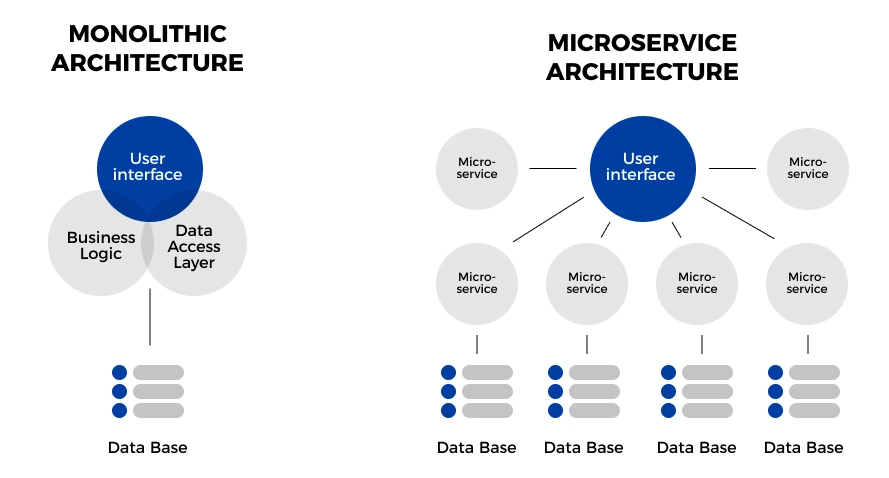
\includegraphics[width=0.9\textwidth]{figures/monolithic_microservices.png}
    \caption{Monolithic vs Microservices Architecture (adapted from~\cite{atlassian_microservices_vs_monolith})}
	\label{fig_background_monolithic_microservices}
\end{figure}

The figure~\ref{fig_background_monolithic_microservices} shows the difference between the monolithic and microservice architecture. In monolithic, all the components of the software system are combined in a single unit whereas in microservice architecture, the whole system is divided into smaller autonomous components. These individual components are easier to manage, scale, maintain and debug.